
\section{Experiments}
\paragraph{Benchmarks.} We evaluated our approach on two challenging, multi-app benchmarks designed to test complex API interactions. \textbf{AppWorld}~\citep{appworld} provides a rigorous testbed of intricate tasks that require agents to coordinate numerous read and write API calls across multiple apps. The environment features 457 APIs distributed across nine everyday apps, with the average task necessitating 10 unique APIs and 45 total calls. AppWorld provides two test splits: \textit{Test-Normal (Test-N)} with 168 tasks and \textit{Test-Challenge (Test-C)} with 417 tasks. The latter introduces two held-out apps to evaluate generalization under increased difficulty. \textbf{OfficeBench}~\citep{wang2024officebench} focuses on office automation, featuring 20 APIs across eight apps. Tasks require agents to plan long-horizon workflows across apps, such as extracting spreadsheet data, scheduling calendar events, and dispatching emails. Following~\citet{li2025simulating}, we excluded OCR-dependent and unsolvable tasks, evaluating on 26 two-app and 46 three-app tasks. 

\paragraph{Models.} We used GLM-4.7-FP8~\citep{glm-4.7} for task synthesis, GLM-5.1-FP8~\citep{glm} for trajectory synthesis (the teacher agent and API simulator), and Gemini-3.1-Pro~\citep{gemini31pro2026} for trajectory filtering. The resulting synthetic data was used to fine-tune eight models: Qwen3 (1.7B, 4B, 8B, and 14B)~\citep{qwen3} and Qwen3.5 (2B, 4B, 9B, and 27B)~\citep{qwen35}.


\paragraph{Training.} Each training trajectory was formatted as a multi-turn conversation consisting of the task instruction, the agent's reasoning and API calls, and the simulated API responses. We followed a standard SFT strategy, training the model to predict the agent's output in each turn conditioned on the task instruction and all previous API calls and their responses. Detailed training hyperparameters are provided in \Cref{sec:app-impl}.

\paragraph{Evaluation.} All results reported in this section are averaged over eight inference runs, with standard deviations presented in \Cref{sec:app-full-results}.

\subsection{Results on AppWorld Benchmark}
\paragraph{\textsc{ESAT} training data from AppWorld APIs.} We generated 9K trajectories using 340 APIs from AppWorld, restricting our selection to seven apps to strictly exclude the two held-out apps in the Test-C split. This dataset is denoted as \textsc{ESAT}-AW7. Further details regarding this dataset can be found in \Cref{app:stats-ESAT-AW7}.

\paragraph{\textsc{ESAT} training data from synthetic APIs.} To increase data diversity, we defined 52 novel synthetic apps with 1017 APIs independent of AppWorld, and used these APIs to generate 6K trajectories. These new apps were created by directly prompting Gemini to generate API specifications covering diverse domains such as e-commerce, productivity, travel, entertainment, and finance. We denote this synthetic app-based dataset as \textsc{ESAT}-S52. Further details regarding app synthesis and dataset statistics are provided in \Cref{sec:synthetic_apps} and \Cref{app:stats-ESAT-S52}. 



\paragraph{AppWorld training data.} The AppWorld dataset provides a training set of 90 tasks. We generated eight trajectories for each task using the GLM-5.1-FP8 model as an agent in the real AppWorld environment, and used the task verifiers included in the dataset to filter for successful trajectories. The resulting 634 trajectories are referred to as the AWT dataset.



\paragraph{Metrics.} Following~\citet{appworld}, we report the task and scenario goal completion (TGC and SGC). Due to space constraints, we present the TGC results in this section and defer the SGC results to \Cref{sec:app-full-results}.

\subsubsection{Effectiveness of \textsc{ESAT} Data} 
\Cref{tab:appworld_main_results} presents the performance improvements achieved by fine-tuning models of various sizes on different training datasets.

\paragraph{Strong generalization to new APIs.} Fine-tuning on the \textsc{ESAT}-S52 dataset, which was generated using 52 synthetic apps independent of AppWorld, results in substantial gains (8.4--47.0\%) across all models. These results confirm that, when seeded with a diverse set of synthetic API specifications, the \textsc{ESAT} pipeline can generate effective training data that imparts robust API-calling skills capable of generalizing to unseen APIs. Notably, for almost all the models (except Qwen3-1.7B), the performance achieved with \textsc{ESAT}-S52 data surpasses that achieved using AWT data collected from the real AppWorld environment, despite \textsc{ESAT}-S52 being generated entirely from synthetic apps.

\begin{table}[t!]
\centering
\small
\begin{minipage}[b]{0.49\linewidth}
\centering
\resizebox{\linewidth}{!}{
\begin{tabular}[b]{lcc}
\toprule
 & \bf{Test-N} & \bf{Test-C} \\
\midrule
\multicolumn{3}{c}{\bf Off-the-shelf models (zero-shot)}\\
\midrule
Gemini-3.1-Pro & 95.3  &  86.8\\
GLM-5.1-FP8  & 86.5 & 81.9 \\
Nemotron-3-120B  & 51.8 & 37.3\\
GPT-4o & 48.8 & 30.2\\
\midrule

\multicolumn{3}{c}{\bf Qwen3-1.7B}\\
\midrule
zero-shot                  & \phantom{0}0.0 & \phantom{0}0.1 \\
\textsc{ESAT-S52} & {15.6} (\textcolor{ForestGreen}{15.6 $\uparrow$}) &  {\phantom{0}8.5} (\textcolor{ForestGreen}{8.4 $\uparrow$}) \\
\textsc{ESAT-S52-AW7} & {24.6} (\textcolor{ForestGreen}{24.6 $\uparrow$}) &  {\phantom{0}9.1} (\textcolor{ForestGreen}{9.0 $\uparrow$})\\
\midrule
\textsc{AWT}                  & 20.0  & {\phantom{0}7.8} \\
\textsc{ESAT-S52-AW7 + AWT} & 27.8 (\textcolor{ForestGreen}{7.8 $\uparrow$}) & 11.9 (\textcolor{ForestGreen}{4.1 $\uparrow$}) \\
\midrule


\multicolumn{3}{c}{\bf Qwen3-4B}\\
\midrule
zero-shot                  & \phantom{0}8.7 & \phantom{0}3.5\\
\textsc{ESAT-S52} & {51.8} (\textcolor{ForestGreen}{43.1 $\uparrow$}) &  {35.9} (\textcolor{ForestGreen}{32.4 $\uparrow$}) \\
\textsc{ESAT-S52-AW7} & {56.9} (\textcolor{ForestGreen}{48.2 $\uparrow$}) &  {34.7} (\textcolor{ForestGreen}{31.2 $\uparrow$})\\
\midrule
\textsc{AWT}                  &  46.7  &  28.3 \\
\textsc{ESAT-S52-AW7 + AWT} & {60.4} (\textcolor{ForestGreen}{13.7 $\uparrow$})  & {40.4} (\textcolor{ForestGreen}{12.1 $\uparrow$})\\
\midrule


\multicolumn{3}{c}{\bf Qwen3-8B}\\
\midrule
zero-shot                  & 21.1 & \phantom{0}7.8\\
\textsc{ESAT-S52} & {59.3} (\textcolor{ForestGreen}{38.2 $\uparrow$}) &  {45.6} (\textcolor{ForestGreen}{37.8 $\uparrow$}) \\
\textsc{ESAT-S52-AW7} & {64.9} (\textcolor{ForestGreen}{43.8 $\uparrow$})  & {49.1} (\textcolor{ForestGreen}{41.3 $\uparrow$})\\
\midrule
\textsc{AWT}                  & 55.7 & 39.1 \\
\textsc{ESAT-S52-AW7 + AWT} & {69.9} (\textcolor{ForestGreen}{14.2 $\uparrow$}) & {54.4} (\textcolor{ForestGreen}{15.3 $\uparrow$}) \\
\midrule


\multicolumn{3}{c}{\bf Qwen3-14B}\\
\midrule
zero-shot                  &  33.2 & 16.3 \\
\textsc{ESAT-S52} & {67.3} (\textcolor{ForestGreen}{34.1 $\uparrow$}) &  {54.4} (\textcolor{ForestGreen}{38.1 $\uparrow$}) \\
\textsc{ESAT-S52-AW7} & 71.7 (\textcolor{ForestGreen}{38.5 $\uparrow$}) & 54.7 (\textcolor{ForestGreen}{38.4 $\uparrow$})\\
\midrule
\textsc{AWT}                  & 67.0  & 44.3 \\
\textsc{ESAT-S52-AW7 + AWT} & 75.2 (\textcolor{ForestGreen}{8.2 $\uparrow$}) & 58.5 (\textcolor{ForestGreen}{14.2 $\uparrow$}) \\
\bottomrule
\end{tabular}
}
\end{minipage}
\hfill
\begin{minipage}[b]{0.49\linewidth}
\centering
\resizebox{\linewidth}{!}{
\begin{tabular}[b]{lcc}
\toprule
 & \bf{Test-N} & \bf{Test-C} \\
\midrule
\multicolumn{3}{c}{\bf Qwen3.5-2B}\\
\midrule
zero-shot                  & \phantom{0}0.1  & \phantom{0}0.2\\
\textsc{ESAT-S52} & {35.5} (\textcolor{ForestGreen}{35.4 $\uparrow$}) &  {26.2} (\textcolor{ForestGreen}{26.0 $\uparrow$}) \\
\textsc{ESAT-S52-AW7} & {46.7} (\textcolor{ForestGreen}{46.6 $\uparrow$}) & {27.9} (\textcolor{ForestGreen}{27.7 $\uparrow$}) \\
\midrule
\textsc{AWT} & 33.2 & 19.1 \\
\textsc{ESAT-S52-AW7 + AWT} & {46.7} (\textcolor{ForestGreen}{13.5 $\uparrow$})  & {27.9} (\textcolor{ForestGreen}{8.8 $\uparrow$}) \\
\midrule



\multicolumn{3}{c}{\bf Qwen3.5-4B}\\
\midrule
zero-shot                  & 27.5 & 17.3\\
\textsc{ESAT-S52} & {64.5} (\textcolor{ForestGreen}{37.0 $\uparrow$}) &  {56.6} (\textcolor{ForestGreen}{39.3 $\uparrow$}) \\
\textsc{ESAT-S52-AW7} & {67.6} (\textcolor{ForestGreen}{40.1 $\uparrow$}) & {60.0} (\textcolor{ForestGreen}{42.7 $\uparrow$})\\
\midrule
\textsc{AWT}                  & 64.3   & 46.7\\
\textsc{ESAT-S52-AW7 + AWT} & {67.6} (\textcolor{ForestGreen}{3.3 $\uparrow$}) & {60.0}  (\textcolor{ForestGreen}{13.3 $\uparrow$}) \\
\midrule

\multicolumn{3}{c}{\bf Qwen3.5-9B}\\
\midrule
zero-shot                  & 25.2  & 15.4 \\
\textsc{ESAT-S52} & {72.2} (\textcolor{ForestGreen}{47.0 $\uparrow$}) &  {61.5} (\textcolor{ForestGreen}{46.1 $\uparrow$}) \\
\textsc{ESAT-S52-AW7} & {75.7} (\textcolor{ForestGreen}{50.5 $\uparrow$}) &  {65.7} (\textcolor{ForestGreen}{50.3 $\uparrow$})\\
\midrule
\textsc{AWT}                 & 71.2 & 53.8 \\
\textsc{ESAT-S52-AW7 + AWT} & {75.7} (\textcolor{ForestGreen}{4.5 $\uparrow$})  &  {65.7} (\textcolor{ForestGreen}{11.9 $\uparrow$})\\
\midrule


\multicolumn{3}{c}{\bf Qwen3.5-27B}\\
\midrule
zero-shot                  & 73.2 & 53.2 \\
\textsc{ESAT-S52} & {83.2} (\textcolor{ForestGreen}{10.0 $\uparrow$}) &  {78.6} (\textcolor{ForestGreen}{25.4 $\uparrow$}) \\
\textsc{ESAT-S52-AW7} & {84.2} (\textcolor{ForestGreen}{11.0 $\uparrow$}) &  {79.0} (\textcolor{ForestGreen}{25.8 $\uparrow$})\\
\midrule
\textsc{AWT}                 & 83.5 & 63.7 \\
\textsc{ESAT-S52-AW7 + AWT} & {84.2} (\textcolor{ForestGreen}{0.7 $\uparrow$})  &  {79.0} (\textcolor{ForestGreen}{15.3 $\uparrow$})\\
\bottomrule
\end{tabular}
}
\end{minipage}
\caption{Performance on AppWorld test splits. For ESAT-S52 and ESAT-S52-AW7, the numbers in parenthesis show the gains with respect to the base model zero-shot performance. For ESAT-S52-AW7 + AWT, they show the gains with respect to AWT. For Qwen3.5 models, using AWT data on top of ESAT data did not give any performance gains. Hence, we report ESAT-S52-AW7 results for ESAT-S52-AW7 + AWT.}
\label{tab:appworld_main_results}
\end{table}


\paragraph{Large gains with minimal target information.}
Fine-tuning on the combined \textsc{ESAT}-S52-AW7 dataset (which merges \textsc{ESAT}-S52 and \textsc{ESAT}-AW7) further improves performance in nearly all settings (up to 11.2\%). The \textsc{ESAT}-AW7 subset provides additional synthetic trajectories generated using minimal target-domain information, relying solely on the API specifications from seven AppWorld apps. 

For all models, fine-tuning on \textsc{ESAT}-S52-AW7 data leads to consistently better performance (0.7--15.3\%) when compared to fine-tuning on AWT data. This demonstrates that highly effective, domain-specific supervision can be generated while entirely bypassing the need for the target environment during training.

Furthermore, fine-tuning on both \textsc{ESAT}-S52-AW7 and AWT data outperforms training solely on AWT data by significant margins (4.1--15.3\%) for the Qwen3 models. For the Qwen3.5 models, augmenting the \textsc{ESAT} data with AWT data does not yield further performance gains. These results establish that the \textsc{ESAT} pipeline provides highly valuable supervision even when real-environment data is available.


\paragraph{Effective knowledge transfer.} 
 When fine-tuned on the \textsc{ESAT}-S52-AW7 dataset, the Qwen3 (8B and 14B) and Qwen3.5 (4B, 9B, and 27B) models outperform the significantly larger GPT-4o~\citep{gpt-4o} and Nemotron-3-120B~\citep{chandiramani2026nemotron} baselines, and the Qwen3.5-27B model achieves a performance that is comparable (< 3\% difference) to the substantially larger GLM-5.1-FP8 teacher model. This demonstrates the efficacy of our approach for knowledge distillation, confirming that complex API-calling capabilities can be transferred to smaller models using purely synthetic, environment-free data.

\paragraph{Generalization to novel user data patterns.} During trajectory generation, our API simulator functions as a digital world model, dynamically simulating the underlying states of a virtual user for the specific task being solved. Consequently, the synthesized data patterns are entirely independent of those in the AppWorld environment. The large performance gains observed on the AppWorld test splits indicate that models trained on \textsc{ESAT} data successfully generalize to unseen user states and data distributions.

\begin{table}[t]
\centering
\small
\resizebox{\linewidth}{!}{%
\begin{tabular}[b]{lcc}
\toprule
 & \bf{2-app} & \bf{3-app} \\
\midrule
\multicolumn{3}{c}{\bf Off-the-shelf models (zero-shot)}\\
\midrule
Gemini-3.1-Pro & 90.0 & 77.7  \\
GLM-5.1-FP8 & 76.7 & 57.1   \\
GPT-4o & 74.5 & 50.9  \\
Nemotron-3-120B & 53.9 & 27.5  \\
\midrule
\multicolumn{3}{c}{\bf LLM-synthesized trajectories - Simia~\citep{li2025simulating} }\\
\midrule
Qwen3-8B Simia & 53.2 & 26.6  \\
Qwen2.5-7B {Simia-RL} & 52.7 & 17.1  \\
\midrule

\multicolumn{3}{c}{\bf Qwen3-1.7B}\\
\midrule
zero-shot & 22.8 & \phantom{0}4.6  \\
\textsc{ESAT-OB} & {52.5} (\textcolor{ForestGreen}{29.7 $\uparrow$}) & {20.7} (\textcolor{ForestGreen}{16.1 $\uparrow$})  \\
\midrule

\multicolumn{3}{c}{\bf Qwen3-4B}\\
\midrule
zero-shot & 49.8 & 38.9  \\
\textsc{ESAT-OB} & {75.7} (\textcolor{ForestGreen}{25.9 $\uparrow$}) & {55.9} (\textcolor{ForestGreen}{17.0 $\uparrow$})  \\
\midrule

\multicolumn{3}{c}{\bf Qwen3-8B}\\
\midrule
zero-shot & 63.2 & 32.7  \\
\textsc{ESAT-OB} & {73.8} (\textcolor{ForestGreen}{10.6 $\uparrow$}) & {55.2} (\textcolor{ForestGreen}{22.5 $\uparrow$})  \\
\bottomrule
\end{tabular}
\hspace{1.5em}
\begin{tabular}[b]{lcc}
\toprule
 & \bf{2-app} & \bf{3-app} \\
\midrule


\multicolumn{3}{c}{\bf Qwen3-14B}\\
\midrule
zero-shot & 69.1 & 47.5 \\
\textsc{ESAT-OB} & {81.9} (\textcolor{ForestGreen}{12.8 $\uparrow$}) & {57.7} (\textcolor{ForestGreen}{10.2 $\uparrow$}) \\
\midrule

\multicolumn{3}{c}{\bf Qwen3.5-2B}\\
\midrule
zero-shot & \phantom{0}9.1 & \phantom{0}0.7 \\
\textsc{ESAT-OB} & {69.6} (\textcolor{ForestGreen}{60.5 $\uparrow$}) & {40.9} (\textcolor{ForestGreen}{40.2 $\uparrow$})  \\
\midrule

\multicolumn{3}{c}{\bf Qwen3.5-4B}\\
\midrule
zero-shot & 62.3 & 37.1 \\
\textsc{ESAT-OB} & {77.0} (\textcolor{ForestGreen}{14.7 $\uparrow$}) & {59.3} (\textcolor{ForestGreen}{22.2 $\uparrow$})  \\
\midrule

\multicolumn{3}{c}{\bf Qwen3.5-9B}\\
\midrule
zero-shot & 68.6 & 46.4  \\
\textsc{ESAT-OB} & {83.6} (\textcolor{ForestGreen}{15.0 $\uparrow$}) & {63.2} (\textcolor{ForestGreen}{16.8 $\uparrow$})  \\

\midrule
\multicolumn{3}{c}{\bf Qwen3.5-27B}\\
\midrule
zero-shot & 84.0 & 64.4  \\
\textsc{ESAT-OB} & {89.7} (\textcolor{ForestGreen}{5.7 $\uparrow$}) & {69.6} (\textcolor{ForestGreen}{5.2 $\uparrow$})  \\
\bottomrule
\end{tabular}
}
\caption{Performance on OfficeBench dataset. The numbers in parenthesis show the gains with respect to the base model zero shot performance.}
\label{tab:officebench_main_results}
\end{table}

\subsection{Results on OfficeBench Dataset}
\paragraph{\textsc{ESAT} training data.} Since OfficeBench is an evaluation-only benchmark without a training set, we generated 1.7K trajectories using 20 APIs from OfficeBench, spanning eight apps. This dataset is denoted as \textsc{ESAT}-OB. Further details regarding this data are provided in \Cref{app:ob-throughput}.

\paragraph{Metric.} Following~\citet{wang2024officebench}, we report the pass rate, defined as the percentage of tasks whose outputs satisfy the customized evaluation function (exact matching, fuzzy matching, or execution-based) associated with each task.


\paragraph{Effectiveness of \textsc{ESAT} data.} \Cref{tab:officebench_main_results} presents the performance gains achieved by training on our environment-free synthetic data. The substantial gains (5.2--60.5\%) once again confirm that highly effective supervision can be generated for API-calling agents while completely bypassing the need for a training environment. Notably, smaller models such as Qwen3-4B and Qwen3.5-4B are able to outperform the much larger Nemotron-3-120B and GPT-4o models. We also outperform Simia~\citep{li2025simulating}, a recent work that focuses on synthetic API-calling data, by a significant margin (20\% or more).

\subsection{LLM Judge Quality}
To understand the effect of the judge model used for trajectory filtering, we performed an ablation study comparing GLM-5.1-FP8 and Gemini-3.1-Pro. \Cref{tab:trajectory_filtering} shows the performance of the Qwen3-8B model trained on ESAT-S52-AW7 data filtered by each of these models. Compared to an unfiltered baseline, employing GLM for trajectory curation actually degrades the performance. In contrast, Gemini proves to be a highly effective filter. By aggressively discarding a larger proportion of low-quality trajectories, it ultimately yields superior downstream performance.



\paragraph{Correlation with real-environment correctness.} To quantify how well our LLM judge corresponds to true executable correctness, we conducted an empirical validation against the real AppWorld environment. We generated 720 trajectories (8 per task across the 90 AppWorld training tasks) using GLM-5.1-FP8 as the agent, and obtained ground-truth trajectory labels from AppWorld's execution-based verifiers. We then re-evaluated these trajectories using our LLM judge, Gemini-3.1-Pro. The judge achieved a precision of 95.2\%, confirming that when our pipeline flags a trajectory as correct, it is highly likely to be genuinely correct. This is the property that matters most for data curation, as it bounds the proportion of erroneous trajectories admitted into the training set.

\begin{figure}[t]
\centering
\small
\setlength{\tabcolsep}{3pt}
\begin{minipage}[b]{0.5\linewidth}
    \centering
    \begin{tabular*}{\linewidth}{@{\extracolsep{\fill}}lccc@{}}
    \toprule
    \textbf{Filter} & \textbf{\#Trajectories} & \textbf{Test-N} & \textbf{Test-C} \\
    \midrule
    No filtering & 19,464 & 61.4  & 39.2 \\
    \midrule
    GLM-5.1-FP8 & 16,966 & 58.5  & 37.1 \\ 
    \midrule
    Gemini-3.1-Pro & 15,617 & \textbf{64.9} & \textbf{49.1} \\
    \bottomrule
    \end{tabular*}
    \captionof{table}{AppWorld performance of Qwen3-8B trained on ESAT-S52-AW7 data filtered with different judge models.}
    \label{tab:trajectory_filtering}
\end{minipage}
\hfill
\begin{minipage}[b]{0.45\linewidth}
    \centering
    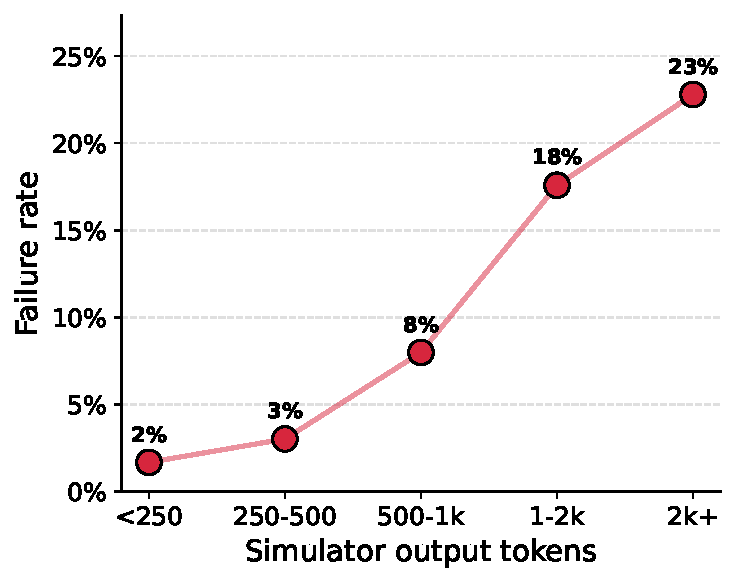
\includegraphics[width=0.8\linewidth]{images/failure_rate_by_output_tokens.pdf}
    \caption{Simulator failure rate as a function of output token length, as judged by GPT-5.1.}
    \label{fig:length}
\end{minipage}
\end{figure}



\paragraph{Agreement with human annotators.} To further validate the trajectory filtering stage, we conducted a human evaluation of our LLM judge. We randomly sampled 200 trajectories (100 accepted and 100 rejected by the judge) and had human annotators assess them using the same grading criteria (see~\Cref{lst:judge_appworld_system}). Annotators disagreed with the judge on only 8 accepted and 2 rejected trajectories, yielding a 95\% overall agreement rate and a Cohen's kappa of 0.90. This near-perfect agreement confirms the high fidelity of our filtering process and, by extension, of our curated \textsc{ESAT} training data.


\begin{table}[t!]
\centering
\small
\begin{minipage}[c]{0.49\linewidth}
\centering
\begin{tabular}[c]{lcc}
\toprule
\bf{Training data} & \bf{Test-N} & \bf{Test-C} \\
\midrule
\multicolumn{3}{c}{\bf Qwen3-4B}\\
\midrule
Zero-shot & 8.7 & 3.5 \\
ToolAlpaca           & 6.3     & 2.0     \\
ToolACE & 9.0 & 3.7\\
Nemotron             & 12.4     &  7.1     \\
% AWT & 46.7 & 28.3 \\
\textsc{ESAT}       &  \bf 56.9 &  \bf 34.7 \\
\midrule
ToolAlpaca + AWT     & 45.8 & 27.2 \\
ToolACE + AWT              & 46.2 & 27.5 \\
Nemotron + AWT       & 47.8 & 27.8 \\
\textsc{ESAT} + AWT & \bf 60.4    & \bf 40.4
\\
\midrule
\multicolumn{3}{c}{\bf Qwen3-8B}\\
\midrule
Zero-shot & 21.1 & 7.8 \\
ToolAlpaca           & 16.9     &  4.9    \\
ToolACE              & 22.2     &  8.8    \\
Nemotron             & 26.8     &  14.4    \\
% AWT & 55.7 & 39.1 \\
\textsc{ESAT}       &  \bf 64.9 &  \bf 49.1 \\
\midrule
ToolAlpaca + AWT     & 54.4 & 31.9 \\
ToolACE + AWT        & 53.1 & 34.1 \\
Nemotron + AWT       & 52.8 & 34.3 \\
\textsc{ESAT} + AWT & \bf 69.9     & \bf  54.4\\
\midrule
\multicolumn{3}{c}{\bf Qwen3-14B}\\
\midrule
Zero-shot & 33.2 & 16.3 \\
ToolAlpaca           & 25.5     & 12.8     \\
ToolACE              & 32.4     & 15.7  \\
Nemotron             & 42.7     &   30.0   \\
% AWT & 67.0 & 44.3 \\
\textsc{ESAT}       &  \bf 71.7 &  \bf 54.7 \\
\midrule
ToolAlpaca + AWT     & 64.2 & 43.4 \\
ToolACE + AWT        & 63.0 & 42.6 \\
Nemotron + AWT       & 62.4 & 44.7 \\
\textsc{ESAT} + AWT & \bf 75.2    & \bf  58.5 \\
\bottomrule
\end{tabular}
\end{minipage}
\begin{minipage}[c]{0.49\linewidth}
\centering
\begin{tabular}[c]{lcc}
\toprule
\bf{Training data} & \bf{Test-N} & \bf{Test-C} \\
\midrule
\multicolumn{3}{c}{\bf Qwen3.5-2B}\\
\midrule
Zero-shot & 0.1 & 0.2 \\
ToolAlpaca           &  0.2    &  0.3     \\
ToolACE              &  0.2    &  0.2    \\
Nemotron             & 0.5     &   0.2   \\
% AWT & 33.2 & 19.1 \\
\textsc{ESAT}   & \bf 46.7 & \bf 27.9 \\
\midrule
ToolAlpaca + AWT     & 33.1 & 16.3 \\
ToolACE + AWT        & 32.2 & 16.1 \\
Nemotron + AWT       & 30.0 & 14.0 \\
\textsc{ESAT} + AWT   & \bf 46.7 & \bf 27.9 \\
\midrule
\multicolumn{3}{c}{\bf Qwen3.5-4B}\\
\midrule
Zero-shot & 27.5 & 17.3 \\
ToolAlpaca           & 25.7     &  17.3     \\
ToolACE              & 20.2     & 10.9     \\
Nemotron             & 26.0     &  17.5    \\
% AWT & 64.3 & 46.7 \\
\textsc{ESAT}   & \bf 67.6 & \bf 60.0 \\
\midrule
ToolAlpaca + AWT     & 58.0 & 39.6 \\
ToolACE + AWT        & 60.2 & 40.0 \\
Nemotron + AWT       & 55.8 & 38.7 \\
\textsc{ESAT} + AWT   & \bf 67.6 & \bf 60.0 \\
\midrule
\multicolumn{3}{c}{\bf Qwen3.5-9B}\\
\midrule
Zero-shot & 25.2 & 15.4 \\
ToolAlpaca           &  24.4    &   15.7   \\
ToolACE              & 18.6     & 12.4     \\
Nemotron             &  31.9    &  20.8    \\
% AWT & 71.2 & 53.8 \\
\textsc{ESAT}   & \bf 75.7 & \bf 65.7 \\
\midrule
ToolAlpaca + AWT     & 69.6 & 51.2 \\
ToolACE + AWT        & 71.4 & 50.3 \\
Nemotron + AWT       & 67.6 & 49.5 \\
\textsc{ESAT} + AWT   & \bf 75.7 & \bf 65.7 \\
\bottomrule
\end{tabular}
\end{minipage}
\caption{Comparison of ESAT-S52-AW7 data with existing synthetic API-calling datasets in terms of effectiveness on AppWorld. When training on a combination of synthetic data and AWT data, we first train on the synthetic data and then further finetune on the AWT data.}
\label{tab:appworld_baseline_comparison}
\end{table}


\subsection{API Simulator Quality Analysis}
\label{sec:simulator_quality}
While the previous section establishes the effectiveness of our simulator-based \textsc{ESAT} pipeline in terms of downstream model performance, this section evaluates the quality of the simulator as a standalone component. To this end, we take 1K successful trajectories generated using AppWorld APIs, comprising approximately 27K simulated API calls. We evaluated the simulated responses of all these calls using GPT-5.1~\citep{openai2025gpt51} as a judge.\footnote{To mitigate potential LLM-as-a-judge bias, we performed the same analysis using another frontier model and observed similar trends. Large-scale human evaluation of such data is prohibitively expensive and time-consuming.} For each API call, the judge was provided with the history of simulated call responses (which was used as the simulator's input context) and validated whether the current simulated response was consistent with the API specification, the call arguments, and the accumulated state from previous calls. According to GPT-5.1, our simulator produced valid responses for 93.7\% of the calls, confirming the high quality of our \textsc{ESAT} training dataset.


\paragraph{Effect of response length.} \Cref{fig:length} \ shows how the simulation failure rate varies with the length of the simulated response. For short responses under 500 tokens, the failure rate remains low (2–3\%), indicating that the simulator reliably produces well-formed responses when the required output is compact. The failure rate then rises steadily with length, reaching 8\% in the 500–1K range, 18\% for 1K–2K tokens, and 23\% beyond 2K tokens. This trend could be due to the inherent limitations of the GLM-5.1-FP8 model used as the simulator in this work, and it could potentially be addressed by using more powerful frontier models that are better at maintaining consistency in long-form generation.

We also investigated the effect of input context length on failure rate and observed no significant correlation.


\begin{table}[t!]
\centering
\footnotesize
\setlength{\tabcolsep}{6pt}
\renewcommand{\arraystretch}{1.1}
% ---------- Table 1: Qwen3 family ----------
\begin{tabular}[b]{lcc}
\toprule
 & \bf{2-app} & \bf{3-app} \\
\midrule
\multicolumn{3}{c}{\bf Qwen3-4B}\\
\midrule
zero-shot   & 49.8 & 38.9 \\
ToolAlpaca  & 11.3 & \phantom{0}2.1 \\
ToolACE     & 15.4 & \phantom{0}3.0 \\
Nemotron    & \phantom{0}8.1 & \phantom{0}0.5 \\
\midrule
ESAT-OB     & \bf 75.7 & \bf 55.9 \\
\midrule
\multicolumn{3}{c}{\bf Qwen3-8B}\\
\midrule
zero-shot   & 63.2 & 32.7 \\
ToolAlpaca  & 29.7 & 10.9 \\
ToolACE     & 29.2 & \phantom{0}5.7 \\
Nemotron    & 52.0 & 35.5 \\
\midrule
ESAT-OB     & \bf 73.8 & \bf 55.2 \\
\midrule
\multicolumn{3}{c}{\bf Qwen3-14B}\\
\midrule
zero-shot   & 69.1 & 47.5 \\
ToolAlpaca  & 30.6 & 12.1 \\
ToolACE     & 37.3 & 22.5 \\
Nemotron    & 70.1 & 45.0 \\
\midrule
ESAT-OB     & \bf 81.9 & \bf 57.7 \\
\bottomrule
\end{tabular}
\hspace{1.5em}
% ---------- Table 2: Qwen3.5 family ----------
\begin{tabular}[b]{lcc}
\toprule
 & \bf{2-app} & \bf{3-app} \\
\midrule
\multicolumn{3}{c}{\bf Qwen3.5-2B}\\
\midrule
zero-shot   & \phantom{0}9.1 & \phantom{0}0.7 \\
ToolAlpaca  & \phantom{0}8.8 & \phantom{0}0.5 \\
ToolACE     & \phantom{0}5.9 & \phantom{0}0.0 \\
Nemotron    & 11.8 & \phantom{0}0.2 \\
\midrule
ESAT-OB     & \bf 69.6 & \bf 40.9 \\
\midrule
\multicolumn{3}{c}{\bf Qwen3.5-4B}\\
\midrule
zero-shot   & 62.3 & 37.1 \\
ToolAlpaca  & 25.3 & \phantom{0}8.0 \\
ToolACE     & 10.3 & \phantom{0}5.2 \\
Nemotron    & 68.2 & 40.7 \\
\midrule
ESAT-OB     & \bf 77.0 & \bf 59.3 \\
\midrule
\multicolumn{3}{c}{\bf Qwen3.5-9B}\\
\midrule
zero-shot   & 68.6 & 46.4 \\
ToolAlpaca  & \phantom{0}7.8 & \phantom{0}0.2 \\
ToolACE     & 36.3 & 11.4 \\
Nemotron    & 73.8 & 49.6 \\
\midrule
ESAT-OB     & \bf 83.6 & \bf 63.2 \\
\bottomrule
\end{tabular}
\caption{Comparison of ESAT-OB data with existing synthetic API-calling datasets in terms of effectiveness on OfficeBench.}
\label{tab:officebench_baseline_comparison}
\end{table}

\subsection{Comparison with Existing Synthetic API-calling Datasets}
We compare the \textsc{ESAT} dataset against three existing synthetic API-calling datasets. The \textbf{ToolAlpaca}~\citep{toolalpaca} and \textbf{ToolACE}~\citep{toolace} datasets target simple API-calling scenarios and do not model a \emph{stateful} environment; specifically, their instances do not require coordinated read/write sequences over an evolving environment state. \textbf{Nemotron}~\citep{chandiramani2026nemotron} is a recent work that scales synthetic API-calling data to 1.5M trajectories, but its API simulator generates each response at the turn level against a correctness rubric rather than a maintained state. Furthermore, its single-and multi-turn scenarios are not designed for the long-horizon, multi-app workflows present in AppWorld and OfficeBench. In contrast, \textsc{ESAT}'s simulator acts as a stateful digital world model that maintains a consistent virtual state across all API calls within a task.


\Cref{tab:appworld_baseline_comparison} and \Cref{tab:officebench_baseline_comparison} compare the effectiveness of these synthetic API-calling datasets in terms of downstream performance on the AppWorld and OfficeBench datasets, respectively. Finetuning models on the ToolAlpaca and ToolACE datasets yields performance that is similar to or worse than the corresponding zero-shot accuracy, while finetuning on the Nemotron dataset leads to only marginal performance gains in some cases. This clearly demonstrates that these simple tool-calling datasets do not equip agents with the skills needed to navigate complex, stateful environments. In contrast, training on the ESAT dataset leads to substantial performance gains on both benchmarks. To test if these alternative synthetic datasets offer useful foundational skills, we further fine-tuned the models on the AWT data collected from the AppWorld environment. Even with this real-environment supervision, their final performance was significantly lower than that of models trained on ESAT data.



% \paragraph{OfficeBench result.} \Cref{tab:officebench_baseline_comparison} shows the same comparison on OfficeBench, where models are fine-tuned on each synthetic dataset and compared against the zero-shot baseline. Here the mismatch is even more pronounced: fine-tuning on ToolAlpaca, ToolACE, or Nemotron data causes severe degradation, often collapsing performance to near zero. For instance, Qwen3-4B drops from a zero-shot score of 49.8 to 11.3 (ToolAlpaca), 15.4 (ToolACE), and 8.1 (Nemotron) on the 2-app split, with the 3-app split falling from 38.9 to 2.1, 3.0, and 0.5, respectively. While the strongest baseline, Nemotron, occasionally matches or slightly exceeds zero-shot on the larger models (\eg, 68.2/40.7 vs. 62.3/37.1 on Qwen3.5-4B), it collapses on the smaller ones, dropping Qwen3-4B to 8.1/0.5. This indicates that training on stateless or short-horizon API-calling data actively harms the long-horizon planning abilities that OfficeBench requires. \textsc{ESAT}-OB, by contrast, delivers large and uniform gains across all models and both splits (\eg, 69.6/40.9 for Qwen3.5-2B and 83.6/63.2 for Qwen3.5-9B), underscoring that faithfully simulating a stateful, multi-app environment is essential for producing effective API-calling supervision.

